\documentclass[article]{article}

\usepackage{mathtools}
\usepackage[utf8]{inputenc}
\usepackage[spanish,es-noshorthands]{babel}
\usepackage{physics}
\usepackage{amsmath}
\usepackage{dcolumn}
\usepackage{bm}
\usepackage{graphicx}
\usepackage{amsfonts}
\usepackage{amssymb}
\usepackage{anysize}
\usepackage{soul}
\usepackage{minted}
\usepackage{dsfont}
\usepackage{color}
\usepackage{pgfplots}
\usepackage{multicol}
\usepackage{cancel}
\usepackage{titlesec}
\usepackage{listings}
\usepackage{color}
\usepackage{lettrine}
\usepackage{float}
\usepackage{longtable}
\usepackage{xparse}
\usepackage[tablename=Tabla]{caption}
\usepackage[backref=page]{hyperref}
\usepackage{titling}
\usepackage{multicol}
\usepackage{subcaption}


\usepackage{multicol}
\setlength{\columnsep}{1cm}

\newcommand{\subtitle}[1]{%
  \posttitle{%
    \par\end{center}
    \begin{center}\large#1\end{center}
    \vskip0.5em}%
}
\providecommand{\abs}[1]{\lvert#1\rvert}
%Encabezado de la tarea%

\title{Caracterización de una película delgada\\mediante el método de Swanepoel} 
%\subtitle{Técnicas de caracterización segundo módulo}

\author{J. A. Rodríguez Franco, J. E. González Balaguera, S. C. Cely Rodríguez}


\date{31 de mayo, 2022}

\begin{document}
\maketitle

\parindent=0cm
\parindent=0.5cm

\titleformat{\section}[hang]
{\normalfont\bfseries}
{\thesection.}{0.5cm}{}
%%%%%%%%%%%%%%%%%%%%%%%%%%%%%%%%%%%%%%%%%%%%%%%%%%%%%%%%%%%%

\begin{multicols}{2}

\section{Introducción.}

    Las películas delgadas son capas finas de un material o aleaciones de diferentes materiales, construidas de manera que adquieran propiedades ópticas o térmicas muy específicas con aplicaciones en la industria y en la ciencia; estas películas delgadas poseen una serie de parámetros importantes que afectan principalmente las propiedades ópticas y por lo tanto se requiere mucha precisión a la hora de diseñarlas y caracterizarlas. 
    
    Es de especial interés poder caracterizar experimentalmente las películas a través de la medición de la transmitancia tanto de la película como del sustrato ya que estos datos permiten obtener información más detallada tal como el índice de refracción, coeficientes de reflexión o extinción, grosor de la película, brechas de energía etc. Sin embargo esta caracterización no es nada sencilla ya que se requiere una gran cantidad de análisis estadístico de datos para obtener la información tan precisa como se quiere, esto junto con diversos modelos matemáticos para diferentes materiales y estructuras da como resultado numerosos métodos de caracterización y entre ellos el método de Swanepoel cuya ventaja radica en que se puede obtener el grosor y el coeficiente $n$ con una precisión de $99\%$, y que basado en el artículo de R. Swanepoel \cite{articulo} se desarrollará más detalladamente en lo sucesivo.
    
    \section{Marco Teórico}
    
    En términos generales, se sabe que la transmitancia de un material está dada por una función compleja de la forma $T=T(\lambda,s, n, d, \alpha)$ pero se puede reducir a una dependencia sencilla respecto al índice de refracción $n(\lambda)$ y a la función de absorbancia $x(\lambda)$ y se modela a través de una función de la forma:
    
    \begin{equation*}
        T=\frac{ax}{b-cx+dx^2}
    \end{equation*}
    
    donde los términos $a,b,c,d$ obviamente dependerán de los parámetros $\lambda,s, n, d, \alpha, k$, sin embargo el poder del método propuesto por Swanepoel radica en realizar varias aproximaciones o simplificaciones que afectan mínimamente las estimaciones de las funciones que se quiere encontrar, basándose únicamente en determinar las curvas envolventes del patrón de difracción de la transmitancia de la película. Para comenzar, la primera aproximación que se realiza es asumir que el sustrato es de longitud infinita, de manera que posteriormente se pueda aplicar la condición $k=0$ la cual es válida en la mayoría del espectro, obteniendo así una función de transmitancia dada por:
    
    \begin{equation}
        T=\frac{Ax}{B-Cxcos(\phi)+Dx^2}
        \label{Eq: Curva transmitancia teorica}
    \end{equation}
    
    con $\phi=4\pi nd/ \lambda$ de forma que al evaluar en los casos extremos en los que hay interferencia, se obtienen las expresiones para las curvas envolventes del espectro en referencia a los puntos coincidentes de máxima y mínima transmitancia respecto al espectro del sustrato.
    
    \begin{equation}
        T_M = \frac{Ax}{B-Cx+Dx^2}
        \label{Eq: Envolvente maxima}
    \end{equation}
    
    \begin{equation}
        T_m = \frac{Ax}{B+Cx+Dx^2}
        \label{Eq: Envolvente mínima}
    \end{equation}
    
    Donde los coeficientes se reducen a:
    
    \begin{table}[H]
        \centering
        \begin{tabular}{|c|c|}
        \hline
            A & $16n^2 s$  \\
            \hline
            B & $(n-1)^3(n+s^2)$\\
            \hline
            C & $2(n^2-1)(n^2-s^2)$\\
            \hline
            D & $(n-1)^3(n-s^2)$\\
            \hline
            x & $e^{-\alpha d}$\\
            \hline
        \end{tabular}
        \caption{Coeficientes de la transmitancia bajo la aproximación de Swanepoel}
        \label{Tab: Coeficientes transmitancia}
    \end{table}
    
    
    Dichos parámetros $A,B,C,D$ son dependientes del índice de refracción y del coeficiente de extinción, por lo tanto, los parámetros buscados se pueden obtener a través de las funciones de las envolventes y por ende, con la identificación de los picos máximos y mínimos
    
    \section{Montaje experimental y medición}
    
    Para comenzar, se tiene una película delgada de grosor $d$ con la propiedad de absorber luz dispuesta sobre un sustrato $s$ transparente como se muestra en la figura \ref{Fig: Diagrama Sustrato} y se hace incidir sobre el sistema un haz de luz con longitud de onda variable de manera que se mide la transmitancia $T$ del sistema Película-Sustrato 
    
    \begin{figure}[H]
    \centering
    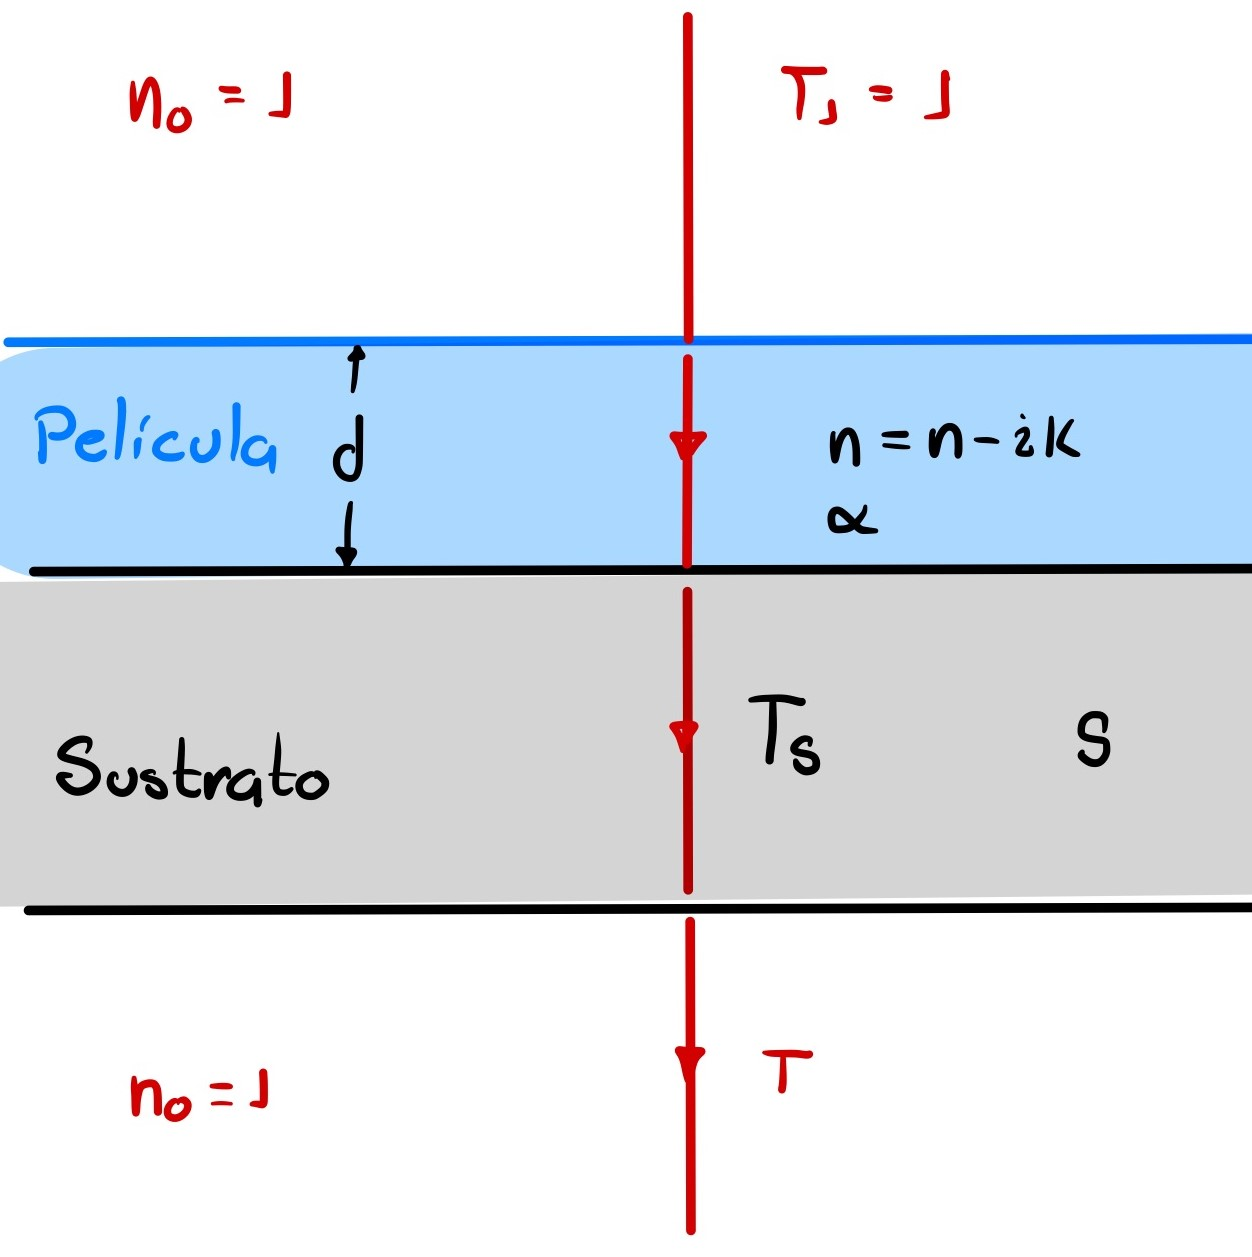
\includegraphics[width= 5cm]{Diagrama Sistema.JPG}
    \caption{Diagrama del sistema película sustrato}
    \label{Fig: Diagrama Sustrato}
    \end{figure}
    
    Dentro de las propiedades de la película, la cantidad de interés es el índice de refracción complejo dado por $\textbf{n}=n-ik$ donde $n$ es el índice de refracción y $k$ el coeficiente de extinción. El coeficiente $k$ se encuentra relacionado con la longitud de onda y el índice de absorción $\alpha$ según la relación \ref{Eq: film Absorption index}:
    
    \begin{equation}
        k=\frac{\alpha}{4}\frac{\lambda}{\pi}
    \label{Eq: film Absorption index}
    \end{equation}

    Por otro lado el sustrato con índice de refracción $s$ y coeficiente de extinción nulo $\alpha_s=0$ (transparente) se escoge de tal manera que su grosor sea mucho mayor que el la película.

    Ahora, el procedimiento experimental consiste como se mencionó anteriormente en hacer incidir distintas longitudes de onda sobre el sistema y medir las trasmitancias del sustrato y del sistema completo de manera que mas adelante se pueda remover la contribución del sustrato en la transmitancia y determinar la transmitancia de la película, ya que con dicha transmitancia se podrá determinar los parámetros ópticos que se buscan. 

    Como resultado de la medición se obtiene un conjunto de datos que arroja la gráfica \ref{Fig: Datos} de transmitancias en función de la longitud de onda, donde la curva azul representa la transmitancia del sustrato y la curva negra da la transmitancia de la película, el perfil de la película presenta picos máximos y mínimos los cuales se dan por efectos de interferencia. También se puede separar los fenómenos de interferencia en tres regiones las cuales se explicarán con más detalle en la sección de análisis de resultados.
    
    \begin{figure}[H]
        \centering
        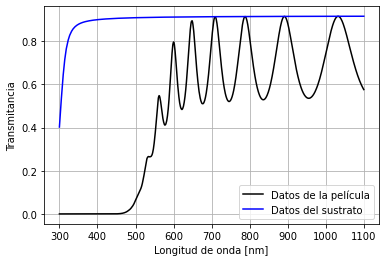
\includegraphics[width= 7cm]{Fig.png}
        \caption{Transmitancias del sustrato y de la película delgada.}
        \label{Fig: Datos}
    \end{figure}
    
    
    \section{Análisis de resultados}
        
        \subsection{Parámetros del sustrato}
    
        De acuerdo a lo sugerido por el método de Swanepoel, primero se calculan las propiedades ópticas del sustrato, con lo cual se usarán las transmitancias en la región $\lambda\geq 700 nm$ puesto que en esta región $T_s$ presenta un valor constante centrado en $T_s\approx 0.915$ y de donde se obtienen el índice de refracción $s$ (Eq \ref{Eq: Indice Refracción sustrato}) y la reflectancia $R$ (Eq \ref{Eq: Reflectancia sustrato})

        \begin{equation}
            s=\frac{1}{T_s}+\left(\frac{1}{T_s^2}-1 \right)^{1/2}=1.534
            \label{Eq: Indice Refracción sustrato}
        \end{equation}

        \begin{equation}
            R=\left(\frac{s-1}{s+1}\right)^2=0.044
        \label{Eq: Reflectancia sustrato}
        \end{equation}
    
        \subsection{Máximos, mínimos e interpolación de curvas envolventes}
    
        Ahora, se deben calcular los coeficientes de refracción para obtener las distancias y los ordenes de interferencia; nótese que no es posible encontrarlas a través de la ecuación de interferencia $2nd=m\lambda$ puesto que no se conocen otros datos distintos de la longitud de onda, pero si es posible usar los picos máximos y mínimos de interferencia para determinar las transmitancias máximas y mínimas dadas por las envolventes y así obtener estos datos faltantes; por lo tanto es de gran ayuda determinar estos picos máximos y mínimos de transmitancia de la película como se muestra en la figura \ref{Fig: Picos de transmitancia}.
    
        \begin{figure}[H]
            \centering 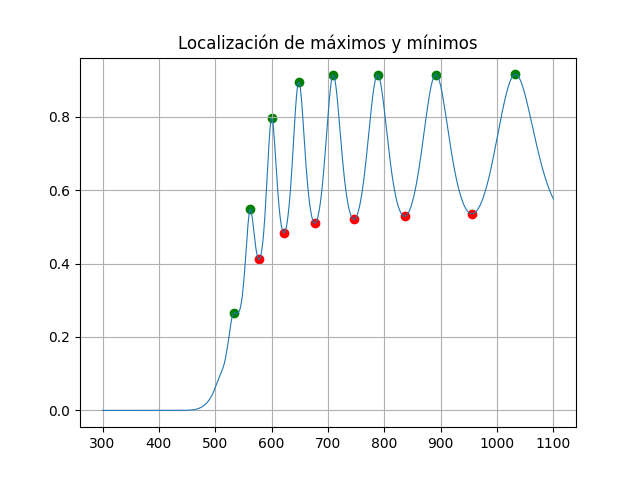
\includegraphics[width=7cm]{minimo_maximo.png}
            \caption{Localización de extremos}
            \label{Fig: Picos de transmitancia}
        \end{figure}
        
        Ahora que se conocen las longitudes de onda correspondientes a los puntos críticos del espectro de transmitancia, se busca obtener el valor de las envolventes para cada una de estas longitudes de onda. Es recomendable realizar una interpolación parabólica con tres puntos, ya que así se garantiza un ajuste suave que nos de valores cercanos a los que buscamos; al realizar esta interpolación encontramos dos puntos asociados a una longitud de onda puesto que las parábolas no siempre se superponen y dan valores ligeramente distintos para cada transmitancia, para resolver esto se toma el promedio de los dos valores dados por las dos parábolas. Repitiendo el proceso para los máximos y los mínimos se obtienen las envolventes interpoladas mostradas en la figura \ref{Fig: Envolventes Interpoladas}
        
        \begin{figure}[H]
            \centering 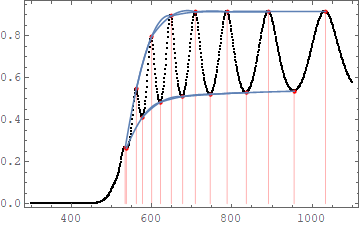
\includegraphics[width=7cm]{Envolventes Interp.png}
            \caption{Interpolación de envolventes superior e inferior}
            \label{Fig: Envolventes Interpoladas}
        \end{figure}
        
        Gracias a este método de interpolación es posible prescindir de los datos iniciales $T(\lambda)$ para trabajar con las envolventes, obteniendo así el conjunto de datos $\{ \lambda_{Max/min}, T_{M}(\lambda), T_{m}(\lambda)\}$ junto con la constante $s$ los cuales son datos suficientes para realizar una primera estimación numérica del índice de refracción $n_1$. 
        
        Como nota final, se discriminan los datos correspondientes a los picos $\lambda_M=1033$ nm y $\lambda_M=534$ nm debido a que al ser el los valores extremos de la lista de picos, no tienen una estimación para la transmitancia mínima dentro de la interpolación.
        
        \subsection{Estimación del índice de refracción $n_1(\lambda)$}
        
        Para encontrar una primera aproximación funcional al índice de refracción, es necesario hacer uso de las relaciones de transmitancia máxima \ref{Eq: Envolvente maxima} y mínima \ref{Eq: Envolvente mínima} teniendo en cuenta que estas ecuaciones se reducen a formas distintas cuando se encuentran en regiones de máxima transmitancia (Región transparente) o mínima transmitancia (Región opaca). A continuación se discuten las regiones y las aproximaciones hechas.
        
        \subsubsection{Región de  transparencia.}
        
        La región transparente comprende aquellas regiones en donde la transmitancia del sustrato es prácticamente constante y por lo tanto la absorción de la película es casi nula. Para esto, el criterio de selección usado es tomar los picos con los cuales la transmitancia del sustrato continúe dentro del intervalo delimitado por $T_s\approx 0.9155 \pm 0.0005$ lo cual corresponde tan sólo a los tres últimos picos, dos máximos y uno mínimo. Aplicando la condición $\alpha=0$ se obtiene que la transmitancia máxima se relaciona con el índice de refracción del sustrato en la forma ya encontrada en la Eq \ref{Eq: Indice Refracción sustrato} mientras que la envolvente mínima lleva a:
        
        \begin{equation*}   T_m=\frac{4n^2s}{n^4+n^2(s^2+1)s^2}
        \end{equation*}
        
        De donde se puede obtener el índice de refracción $n$ de forma analítica con la expresión \ref{Eq: n transparencia} 
        
        \begin{equation}
            n=\sqrt{M+\sqrt{M^2-s^2}}
            \label{Eq: n transparencia}
        \end{equation}
        
        con $M=\frac{2s}{T_m}-\frac{s^2+1}{2}$
    
        \subsubsection{Región de absorción débil y media.}
        
        La región de absorción media-débil son las regiones donde la absorción presentada no es tan fuerte para disminuir significativamente la transmitancia \footnote{Una disminución significativa en este contexto implica transmitancias del orden de $T\leq 0.6$, es decir, los picos por debajo de los $600$ nm para este caso} y, por lo tanto, se describen bajo las condiciones $\alpha\neq0$ y $x<1$. Para la determinación del índice de refracción en esta región se necesitan los valores de las dos envolventes $T_M$ y $T_m$ y se usa la Eq \ref{Eq: n región media}
        
        \begin{equation}
            n=\sqrt{[N+\sqrt{(N^2-s^2)}]}
            \label{Eq: n región media}
        \end{equation}
         
        Donde el parámetro $N$ está dado por la ecuación $N=2s\left[\frac{T_M-T_m}{T_M*T_m}\right]+\frac{S^2+1}{2}$
        
        
        \subsubsection{Región de absorción fuerte}
        
        El análisis de esta región afortunadamente no es relevante para el cálculo de los coeficientes de interés, sin embargo eventualmente los picos de esta región pueden servir para comprobar que todas las funciones $T(\lambda)$ convergen a un valor específico.
        
        
        \subsubsection{Función $n(\lambda)$}
        
        Gracias al análisis de las anteriores tres regiones y la discriminación de datos, se obtiene un conjunto de datos $\{ \lambda, T_m(\lambda), T_M(\lambda), n_1(\lambda)\}$ en un intervalo de longitudes de onda $\lambda\in [600,1000]$ nm representado en las tres primeras columnas de la tabla \ref{tab: Datos Refraxión y Película}; con estos datos es posible graficar el comportamiento funcional del índice de refracción el cual sugiere una función dependiente del inverso cuadrado de la longitud de onda (figura \ref{fig: n_1 for peaks}). 
        
        \begin{figure}[H]
        \centering
        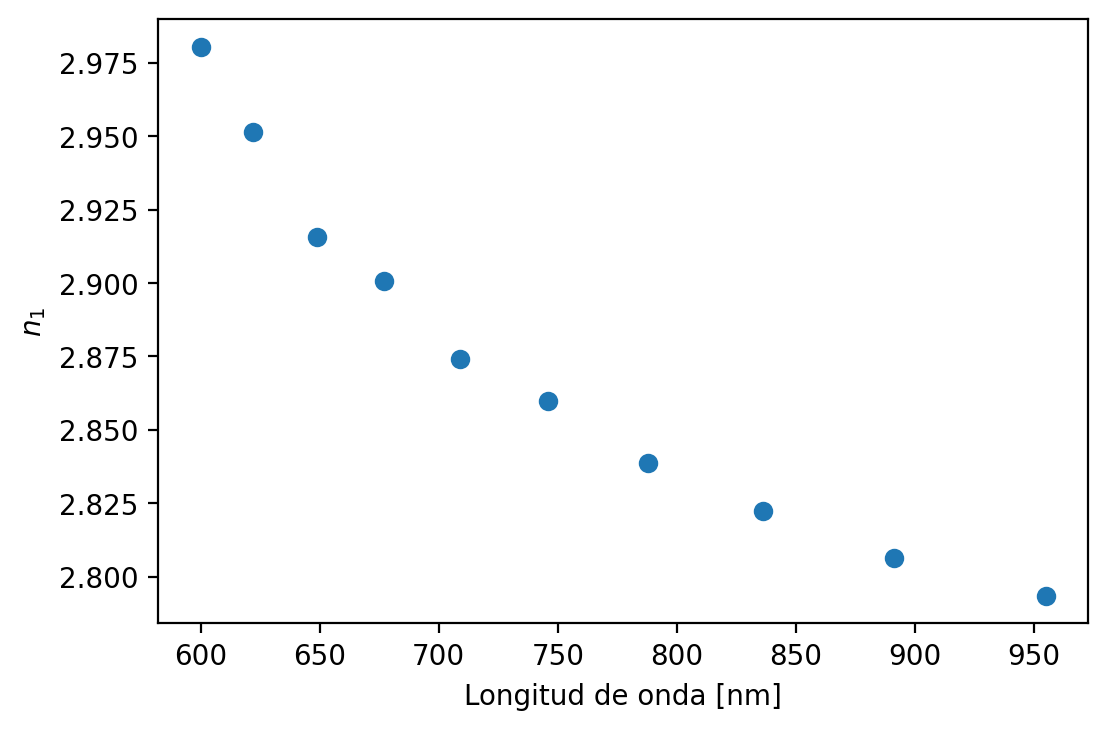
\includegraphics[width=7cm]{n_1 data.png}
        \caption{Estimación del índice de refracción para los picos}
        \label{fig: n_1 for peaks}
        \end{figure}
        
        Cuando se realiza la gráfica $n$ Vs $1/\lambda^2$ se observa más claramente el comportamiento lineal descrito por el ajuste \ref{Eq: First linear fit n} y mostrado en la figura \ref{fig: n_1 linear fit}
        
        \begin{figure}[H]
        \centering
        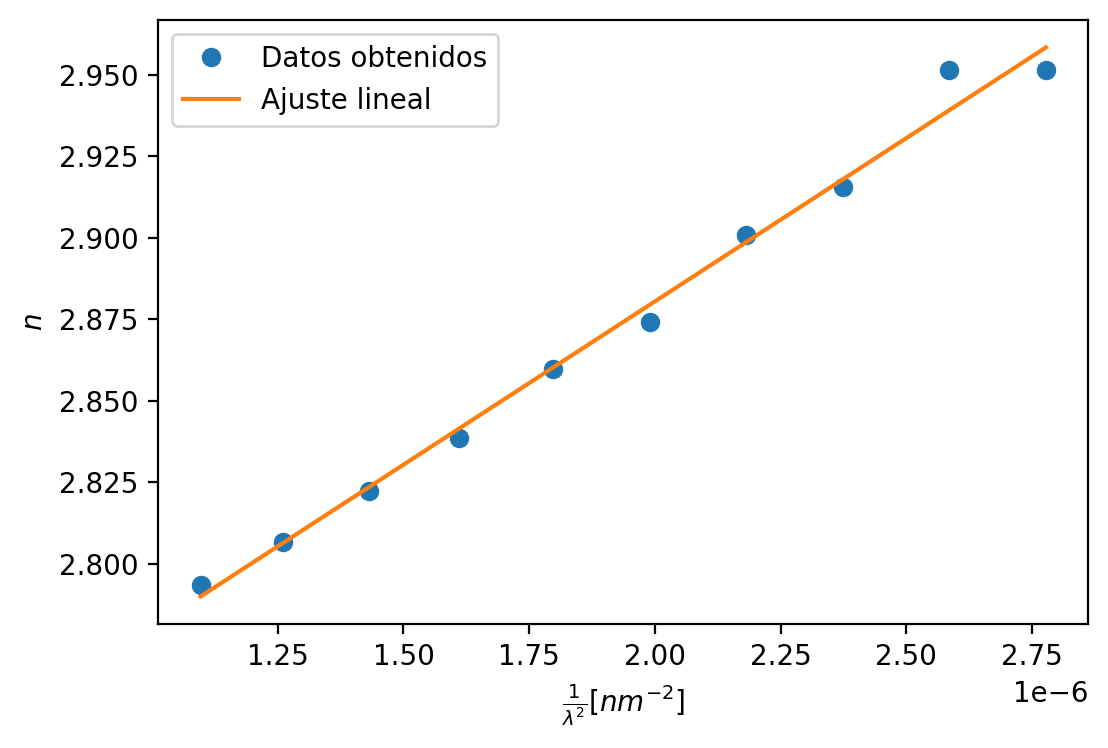
\includegraphics[width=7cm]{n_1 linear fit.png}
        \caption{Ajuste lineal para $n$}
        \label{fig: n_1 linear fit}
        \end{figure}
        
        \begin{equation}
            n_1(\lambda)=\frac{1.001 \times 10^{5} (nm^2)}{\lambda^2}+2.6801
            \label{Eq: First linear fit n}
        \end{equation}
        
        con un coeficiente de correlación, $R^2=0.9912$ lo que en principio nos dice que el modelo lineal es una buena aproximación funcional para los datos obtenidos
        
        \subsection{Determinación del grosor de la película y los órdenes de magnitud}
        
        De igual manera que el índice de refracción, con los datos de la sección anterior es posible hacer una estimación del grosor de la película utilizando la expresión \ref{Eq: Thickness} donde los subíndices indican que los picos deben ser máximos sucesivos o mínimos sucesivos. Los valores encontrados para cada par de datos se muestran en la quinta columna de la tabla \ref{tab: Datos Refraxión y Película}
        
        \begin{equation}
            d=\frac{\lambda_1 \lambda_2}{2(\lambda_1 n_2 - \lambda_2 n_1)}
            \label{Eq: Thickness}
        \end{equation}
        
        de manera que al realizar un promedio estadístico de estos valores junto con la desviación estándar arrojan una estimación del grosor $\Bar{d}_1=1100\pm24$ nm.
        
        Gracias a este valor central que se tiene para el grosor es posible determinar los órdenes de interferencia para cada longitud de onda con ayuda de la ecuación:
        
        \begin{equation}
            m=\frac{2nd}{\lambda}
            \label{Eq: Patron Interferencia}
        \end{equation}
        
        donde $m$ es un número entero para las transmitancias máximas y es un número de la forma $n+1/2$ para las transmitancias mínimas.

        \subsection{Correcciones al coeficiente de refracción y al grosor de la película}
        
        En este punto se podría afirmar que ya se tienen dos de los parámetros importantes para caracterizar la película; sin embargo aún carecen de un refinamiento porque presentan dispersión de errores. El refinamiento que se les puede realizar es bastante sencillo, ya que las primeras estimaciones de $n_1(\lambda)$ y $\Bar{d}_1$ tenían como objetivo verificar que se está trabajando bajo los órdenes de interferencia correctos y de esta manera redondear estos valores a cantidades exactas. Una vez obtenidos los ordenes de interferencia se recalculan las estimaciones del grosor para cada longitud de onda usando nuevamente la ecuación \ref{Eq: Patron Interferencia} y los valores exactos de $m$, la función \ref{Eq: First linear fit n} y la longitud de onda; con esto se obtienen unos grosores $d_2$ menos dispersos que los $d_1$ y al repetir el proceso de obtener el promedio y la desviación estándar se obtiene un valor definitivo dado por:
        
        \begin{equation}
            \Bar{d}_2=1109\pm 2 nm
        \end{equation}
        
        El cual es un valor mucho más preciso que el primero que se había obtenido. De la misma manera se repite el cálculo para la refracción y se realiza una nueva regresión lineal para obtener su forma funcional:
        
        \begin{equation}
            n_2(\lambda)=\frac{1.035\times10^5}{\lambda}+2.6765
            \label{Eq: n2 Refractive index}
        \end{equation}
        
        
        \subsection{Determinación de $x(\lambda)$, $\alpha (\lambda)$ y $k(\lambda)$}
        
        Una vez obtenida la función \ref{Eq: n2 Refractive index} que representa el índice de refracción de la película, podemos hacer uso de diferentes curvas de transmitancia, tales como las transmitancias máxima $T_M$ y mínima $T_m$, la transmitancia que pasa por los puntos de inflexión $T_i=(2T_MT_m)/(T_M+T_m)$ o la media geométrica de la transmitancia $T_{\alpha}=\sqrt{T_MT_m}$; dependiendo la cantidad escogida se tienen distintos métodos matemáticos para obtener la absorbancia $x$. En este caso por sugerencia del autor se escoge el método que usa la envolvente mayor, el cual usa la ecuación \ref{Eq: absorbancias x}
        
        \begin{equation}
            x=\frac{E_M-\sqrt{E^2_M-(n^2-1)^3(n^2-s^4)}}{(n-1)^3(n-s^2)}
            \label{Eq: absorbancias x}
        \end{equation}
        
        donde $E_M=\frac{8n^2s}{T_M}-(n^2-1)(n^2-s^2)$. Este método también funciona para la envolvente mentor reemplazando $T_M$ por $T_m$, de igual manera se puede usar el método $T_i$ usando la misma expresión para $x$ y reemplazando $E_M$ por $F=8n^2s/T_i$. En las figuras \ref{fig: x-general} y \ref{fig: x T_M} se ilustran los resultados para esta función de absorbancia usando tanto las envolventes como la transmitancia de inflexión.
        
        \begin{figure}[H]
        \centering
        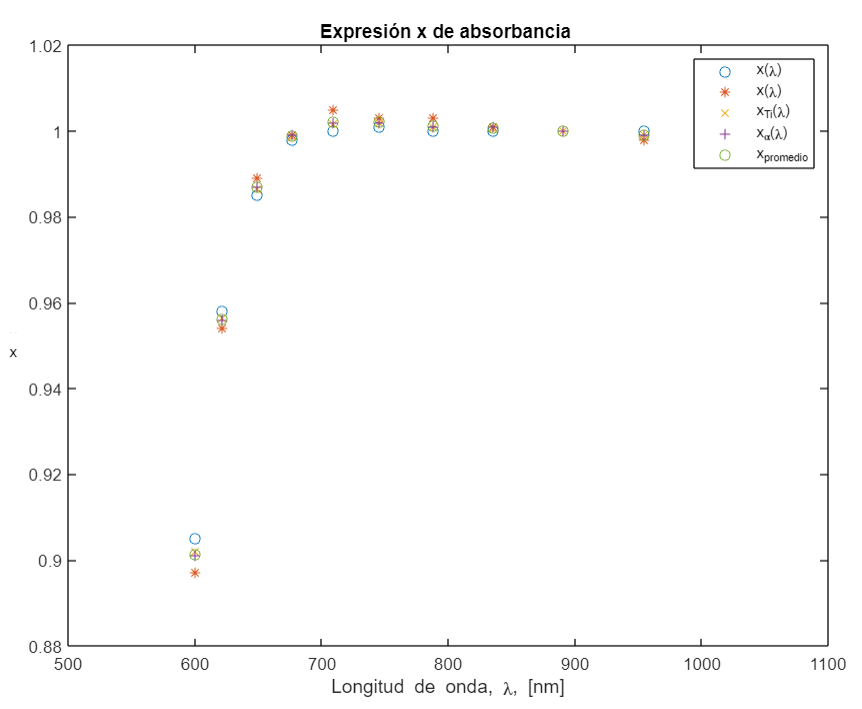
\includegraphics[width=7cm]{valores-x.png}
        \caption{Valores de $x$ calculados con las transmitancias $T_M$, $T_m$, $T_i$, $T_i$ y $T_{\alpha}$}
        \label{fig: x-general}
        \end{figure}
        
        \begin{figure}[H]
        \centering
        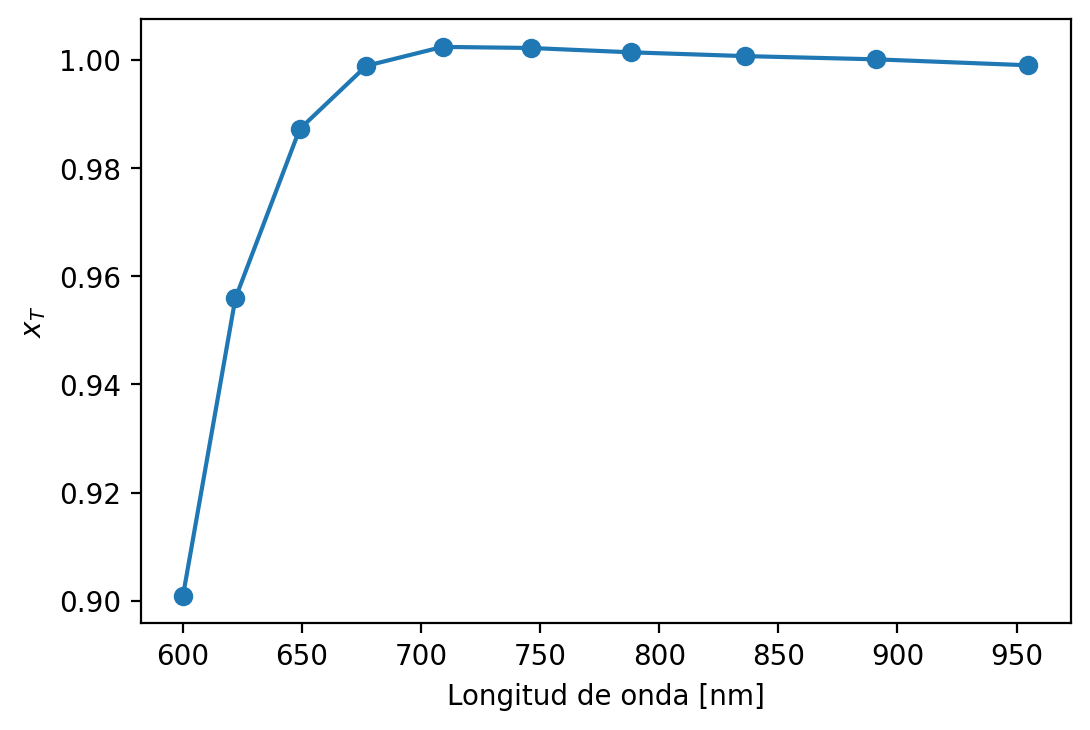
\includegraphics[width=7cm]{x T_M.png}
        \caption{Curva de tendencia para los valores de $x$ obtenidos a través de $T_M$}
        \label{fig: x T_M}
        \end{figure}
        
        Nótese que para determinar $x$ se requiere conocer $\lambda,s,n$ lo cual ya se tiene, por lo tanto no se requiere más para tener la función $x$. Ahora con esta información se puede encontrar fácilmente el índice de absorción $\alpha(\lambda)$ usando el modelo teórico de la tabla \ref{Tab: Coeficientes transmitancia} con lo que se obtiene \ref{Eq: Alpha}
        
        \begin{equation}
            \alpha=-\frac{Ln(x)}{d}
            \label{Eq: Alpha}
        \end{equation}
        
        de la misma manera que con $x$, en las figuras \ref{fig: valores alpha} y \ref{fig: alpha T_M} se ilustran los resultados del índice de absorción. 
        
        \begin{figure}[H]
        \centering
        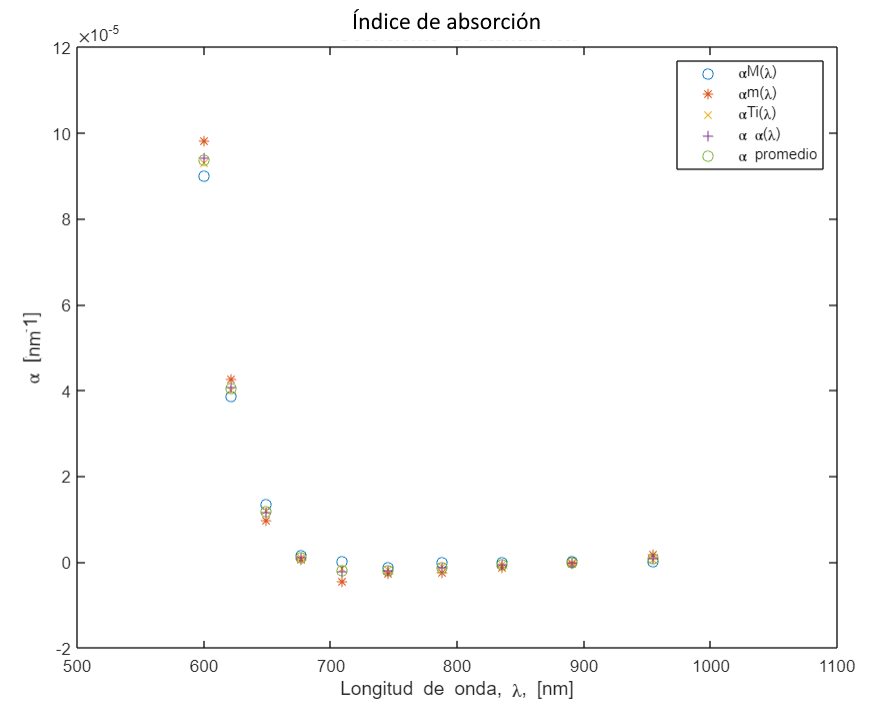
\includegraphics[width=7cm]{valores-alpha.png}
        \caption{Valores de $\alpha$ calculados con las transmitancias $T_M$, $T_m$, $T_i$, $T_i$ y $T_{\alpha}$}
        \label{fig: valores alpha}
        \end{figure}
        
        \begin{figure}[H]
        \centering
        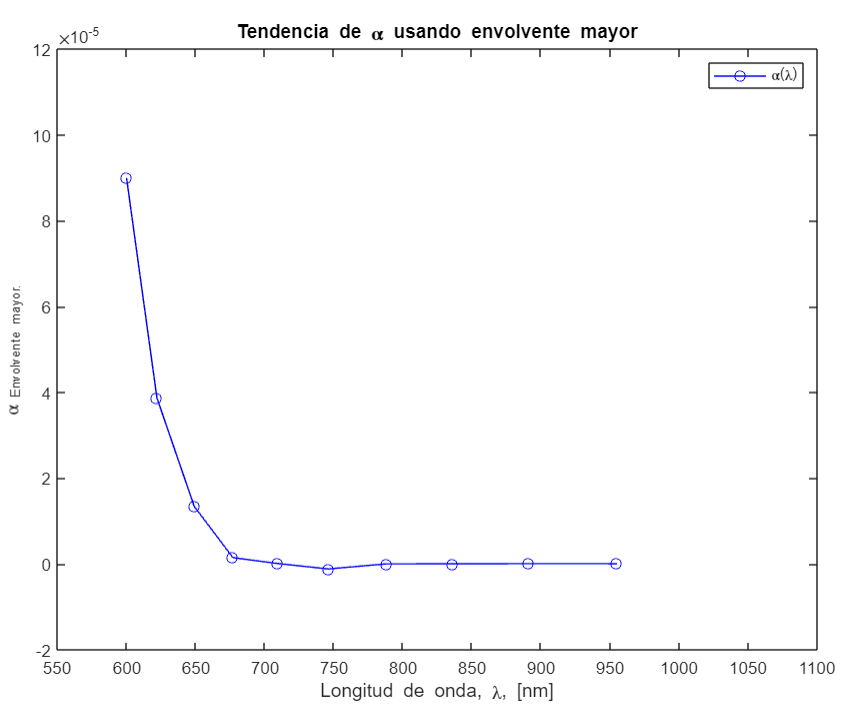
\includegraphics[width=7cm]{alpha T_M.png}
        \caption{Curva de tendencia para los valores de $\alpha$ obtenidos a través de $T_M$}
        \label{fig: alpha T_M}
        \end{figure}
        
        De alguna manera se intuye una figura que evoca una función similar a una exponencial que decae, por lo cual se podría graficar $ln(\alpha)$ para determinar si tiene alguna relación funcional clara con $\lambda$; de hecho, el artículo sugiere que la función $ln(\alpha)$ suele presentar comportamientos de la forma $ln(\alpha)=\frac{c_1}{\lambda^2}+c_2$ sin embargo al realizar esta gráfica se encontraron principalmente dos problemas:
        
        \begin{itemize}
            \item La función $\alpha$ posee unos cuantos valores negativos (posiblemente por causa de la propagación de errores en el proceso de cálculo) de manera que no es posible obtener el logaritmo de estos valores.
            
            \item Si se discriminan los valores que no se pueden calcular y se grafican los restantes, el perfil obtenido no posee una tendencia lineal sino cuadrática, por lo cual no se expresa esta forma funcional debido a que puede llevar a grandes discrepancias a la hora de realizar el perfil simulado con los parámetros obtenidos hasta el momento.
        \end{itemize}
         
        
        Finalmente, con los valores obtenidos de $\alpha$ se puede encontrar fácilmente $k$ usando la ecuación \ref{Eq: film Absorption index} de manera que se completa la caracterización de los parámetros ópticos buscados en la película delgada. Los datos obtenidos se pueden encontrar en la tabla \ref{tab: Datos x,alpha,k} mientras que la gráfica obtenida se puede observar en \ref{fig: Extintion Data}
        
        \begin{figure}[H]
        \centering
        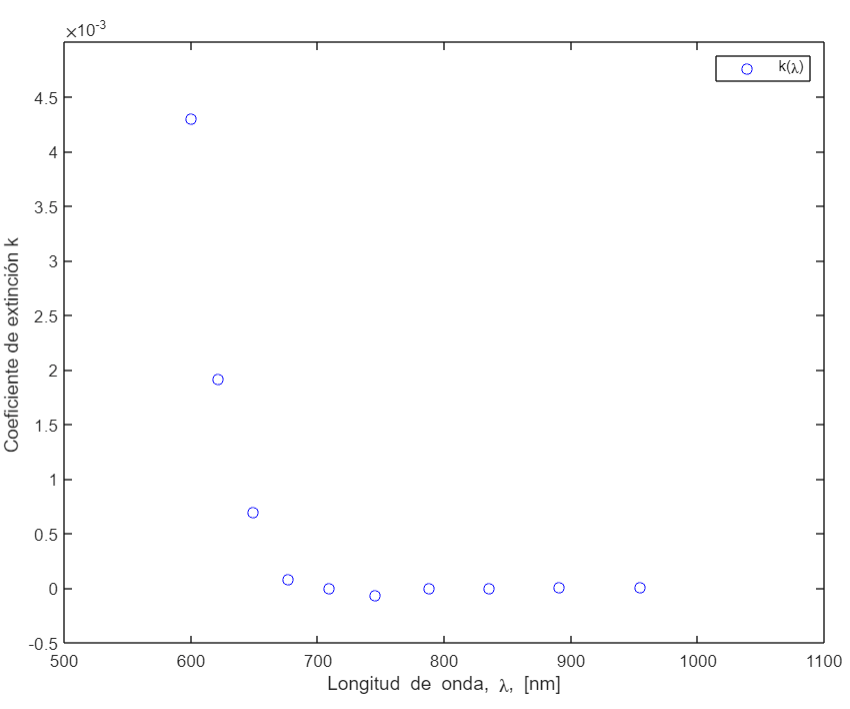
\includegraphics[width=7cm]{extincion-coefficient.png}
        \caption{Valores del coeficiente de extinción en función de la longitud de onda.}
        \label{fig: Extintion Data}
        \end{figure}
        
    \section{Comparación del espectro experimental y el modelo numérico}
     
    De acuerdo al modelo teórico descrito por las ecuaciones \ref{Eq: Curva transmitancia teorica}, \ref{Eq: Envolvente maxima}, \ref{Eq: Envolvente mínima} y los parámetros \ref{Tab: Coeficientes transmitancia} ya se tienen las cantidades necesarias para determinar el perfil teórico de la curva de transmitancia del material, así como de las envolventes; estos parámetros son $s$, $n$, $d$ y $\alpha$ de manera que podemos realizar la comparación de los datos y del perfil teórico para determinar qué tan correctas son las caracterizaciones hechas. Además de usar las ecuaciones teóricas, se hizo uso de una simulación usando programación orientada a objetos, con el fin de facilitar la aplicación de los múltiples métodos de las ecuaciones descritas y hallar las constantes ópticas en las regiones a considerar.
    
    \subsection{Envolventes}
        
        Para hallar los picos de máximos y mínimos se hizo uso de la función de findpeaks de Matlab y aplicando los parámetros encontrados se obtiene el perfil de las envolventes mostrado en la figura \ref{fig:envolventes-matlab}

        \begin{figure}[H]
        \centering
        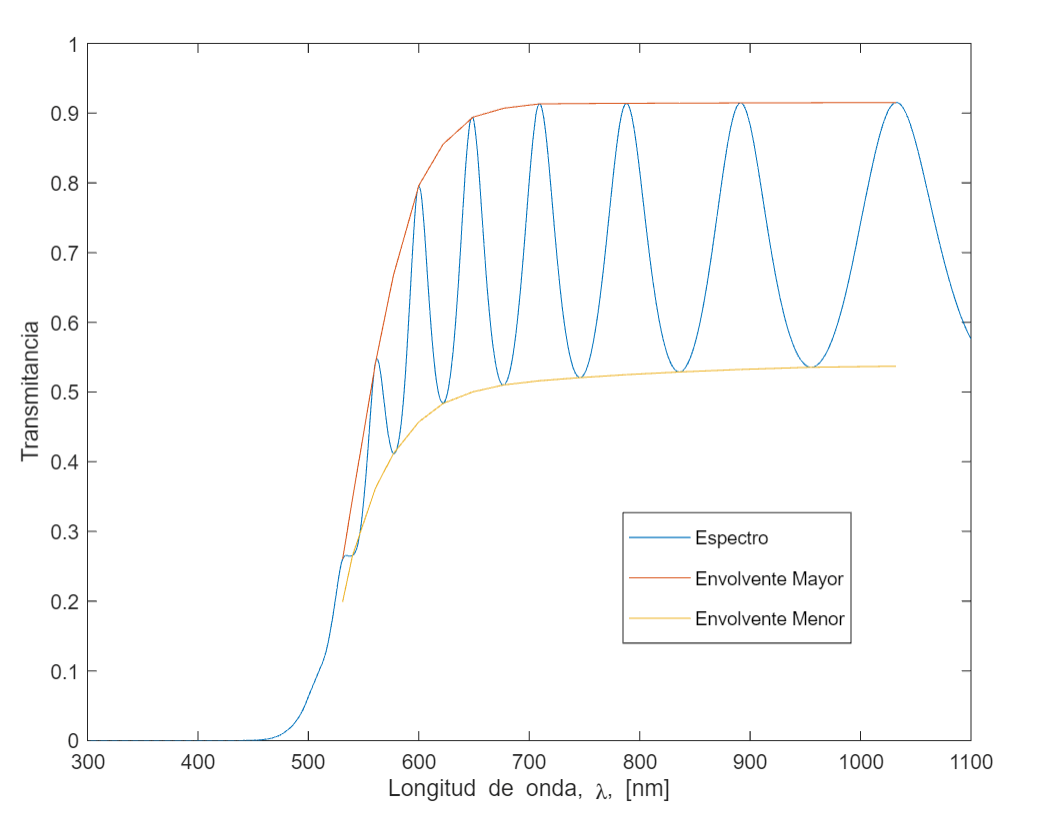
\includegraphics[width=7cm]{envolventesMym.png}
        \caption{Envolvente mayor y menor en función de $\lambda$   función Findpeaks}
        \label{fig:envolventes-matlab}
        \end{figure}
        
    \subsection{Comprobación de los parámetros ópticos}   
    
        En un primer acercamiento, se obtuvo una curva para el modelamiento teórico usando interpolación sobre máximos y mínimos, sin embargo, el valor de la distancia calculado resulto no ser acorde al experimento, como se percibe al superponer  la simulación numérica sobre los datos base. En la figura \ref{fig:ajuste-sin-correcciones} se observa un  desfase de los picos que se acentúa en la zona de transparencia, lo cual indica que posiblemente en el algoritmo hay un error de estimación con algunos valores. 
        \begin{figure}[H]
            \centering 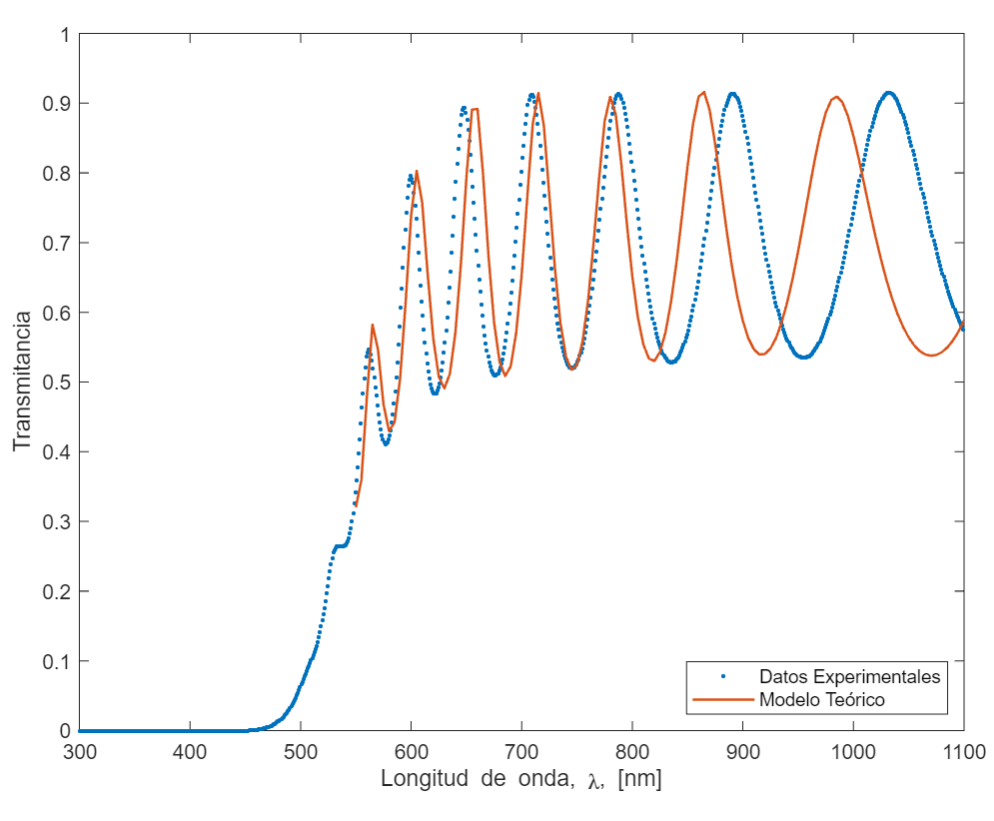
\includegraphics[width= 7cm]{ajuste.png}
            \caption{Curva de simulación numérica sin correciones} \label{fig:ajuste-sin-correcciones}
        \end{figure}
        
        Haciendo un uso directo de los parámetros calculados y las formas funcionales de $n$ y $\alpha$ Se procedió a recalcular los valores de las constantes ópticas por regiones, revisando posibles desviaciones por aproximación o errores de tipado. Se ajustó manualmente el rango de longitud de onda con lo cual se obtuvo un mejor ajuste respecto a la curva experimental, como se evidencia en la figura \ref{fig:ajuste}.
        

        \begin{figure}[H]
            \centering 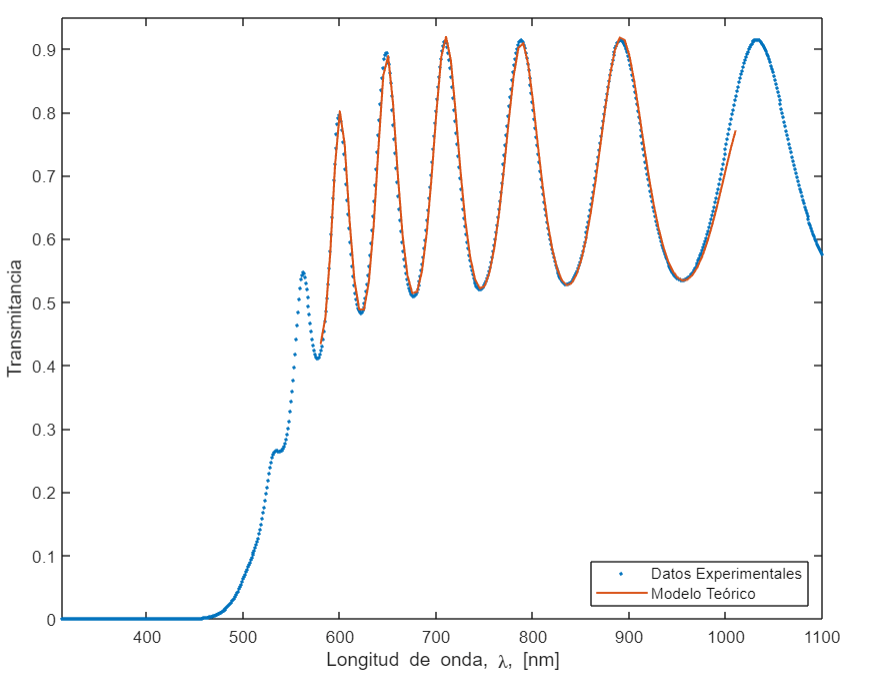
\includegraphics[width= 7cm]{simulacion.png}
            \caption{Curvas de ajuste para región media débil}
            \label{fig:ajuste}
            \end{figure}
        
    Como se puede observar, la región del ajuste fue restringida únicamente a la zona en la cual se tomaron datos de los picos sin extrapolar la curva a las zonas de los datos que no se tomaron, lo cual nos muestra una coincidencia mucho más precisa, indicando que la caracterización de los parámetros es correcta dentro de la zona analizada.
   
    \section{Bonus track: Determinación del Gap de energía}
        
        Con todos los datos obtenidos hasta el momento no sólo se caracteriza el material, también es posible obtener información acerca de los gaps de energía y así determinar las transiciones del material.
        
        Para esto se utiliza la teoría de Tauc que describe la interacción radiación-materia para determinar la brecha de energía de este material amorfo en forma de película con ayuda de la ecuación:
        
        \begin{equation}
            (\alpha h v)^n=A(hv-E_g)
        \end{equation}
        
        donde: 
        
        El exponente $n$ describe el tipo de transición de energía que se da en la brecha.
        
        \begin{itemize}
            \item $n=2$ para transiciones directas permitidas
            \item $n=2/3$ para transiciones directas prohibidas
            \item $1/2$ para transiciones indirectas permitidas
            \item $n=1/3$ para transiciones indirectas prohibidas 
        \end{itemize}
        
        la cantidad $E_g$ determina un punto de corte para una recta y determina la energía correspondiente a la brecha
        
        debido a que se tienen los datos de la longitud de onda, se usa la relación $\nu=c/\lambda$ para obtener la dependencia funcional adecuada mostrada en la ecuación \ref{Eq: Tauc}
        
        \begin{equation}
            \alpha^n\Big( \frac{hc}{\lambda}\Big)^n=A\Big(\frac{hc}{\lambda}-E_g\Big)
            \label{Eq: Tauc}
        \end{equation}
        
        Una vez realizados los gráficos se encuentra que los cuatro presentan regiones lineales, de manera que al realizar la regresión para cada uno de los exponentes se obtiene la siguiente tabla:
        
        \begin{table}[H]
            \centering
            \begin{tabular}{|c|c|c|}
            \hline
            Transiciones & Permitida & Prohibida \\ 
            \hline
            Directa & 5,34 & 4,81  \\     
            \hline
            Indirecta & 4,01 & 5,64  \\ \hline
            \end{tabular}
            \label{Tab: Gap values and transitions}
            \caption{Transiciones y valores de la energía de las brechas en unidades de $eV$.}
        \end{table}
        \end{multicols}
        \newpage
        
        \begin{figure}[H]
            \centering
            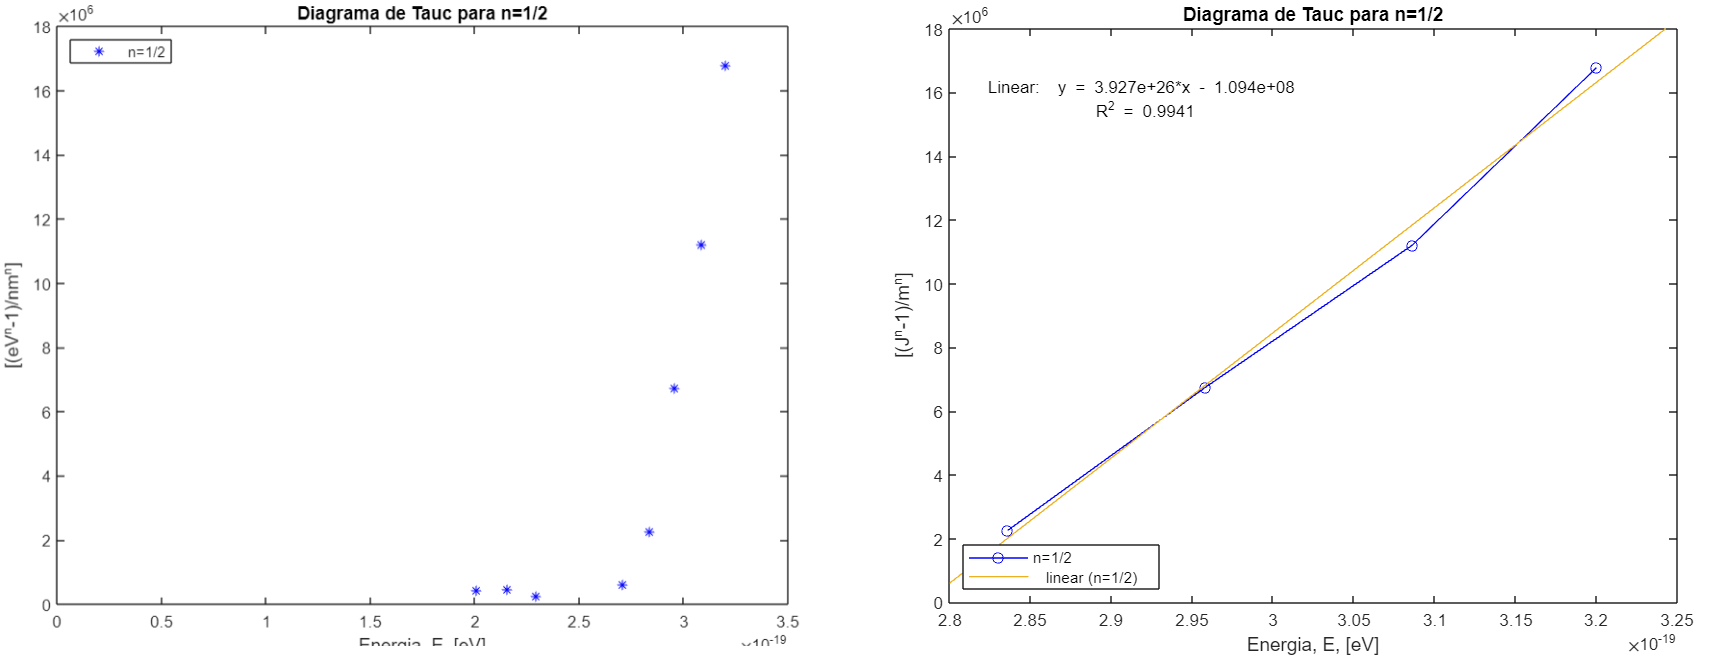
\includegraphics[width=0.75\linewidth]{1_2-gap.png}
            \caption{ Diagrama de Tauc para exponente $ n=\frac{1}{2}$. La función de regresión corresponde a $y=3.927e+26x-1.094\times10^{8}$ y tiene coeficiente de correlación $R^2=0.9941$.}
            \label{fig:gap 1}
        \end{figure}
    
    \begin{figure}[H]
        \centering
        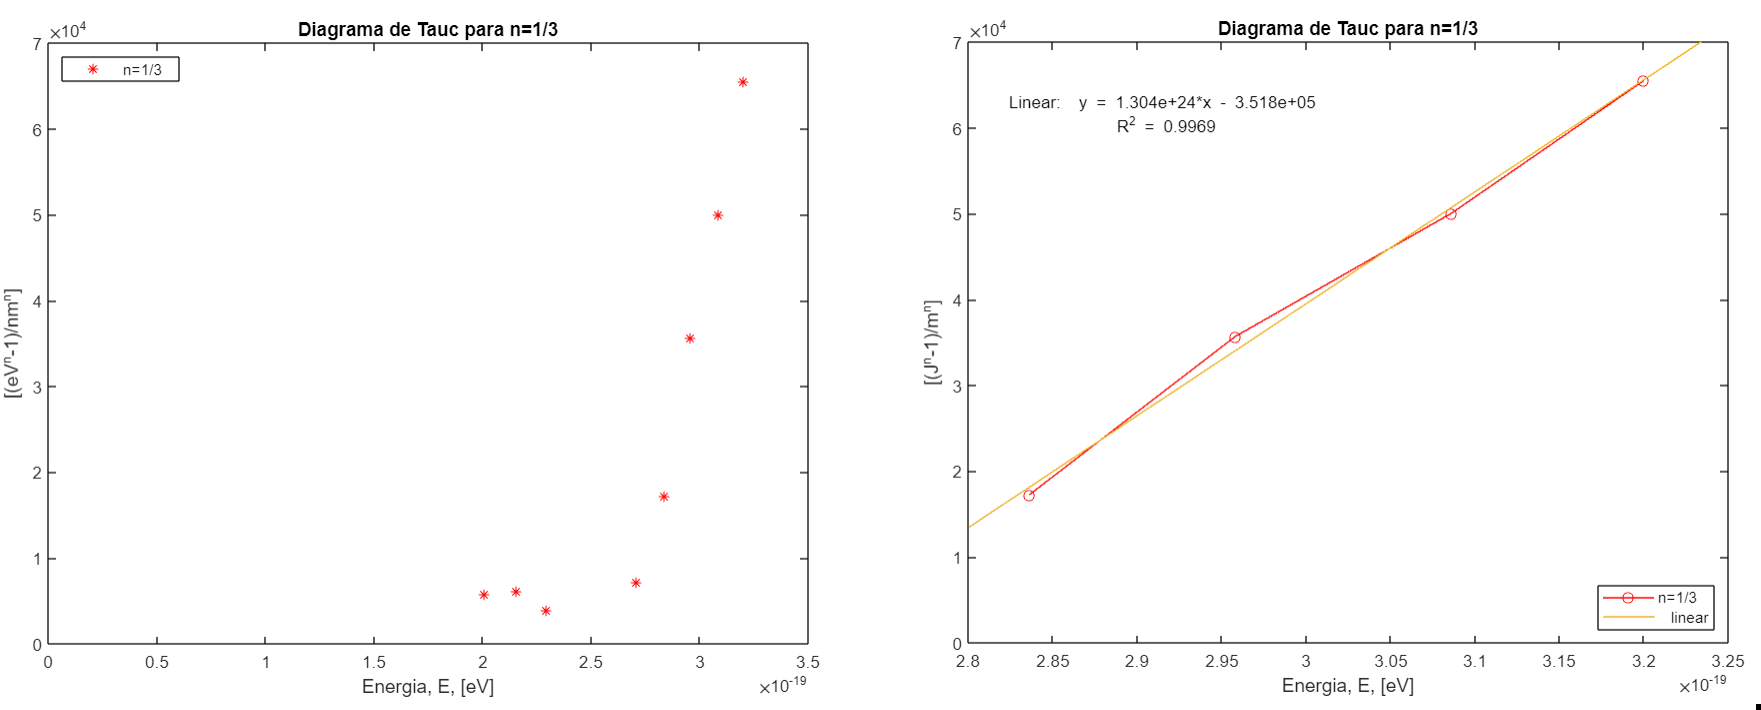
\includegraphics[width=0.75\linewidth]{1_3-gap.png}
            \caption{ Diagrama de Tauc para exponente $ n=\frac{1}{3}$.  La función de regresión corresponde a $y=1.304e+24x-3.518\times10^{5}$ y tiene coeficiente de correlación $R^2=0.9969$.}
        \label{Fig:gap 2}
    \end{figure}
    
    \begin{figure}[H]
        \centering
        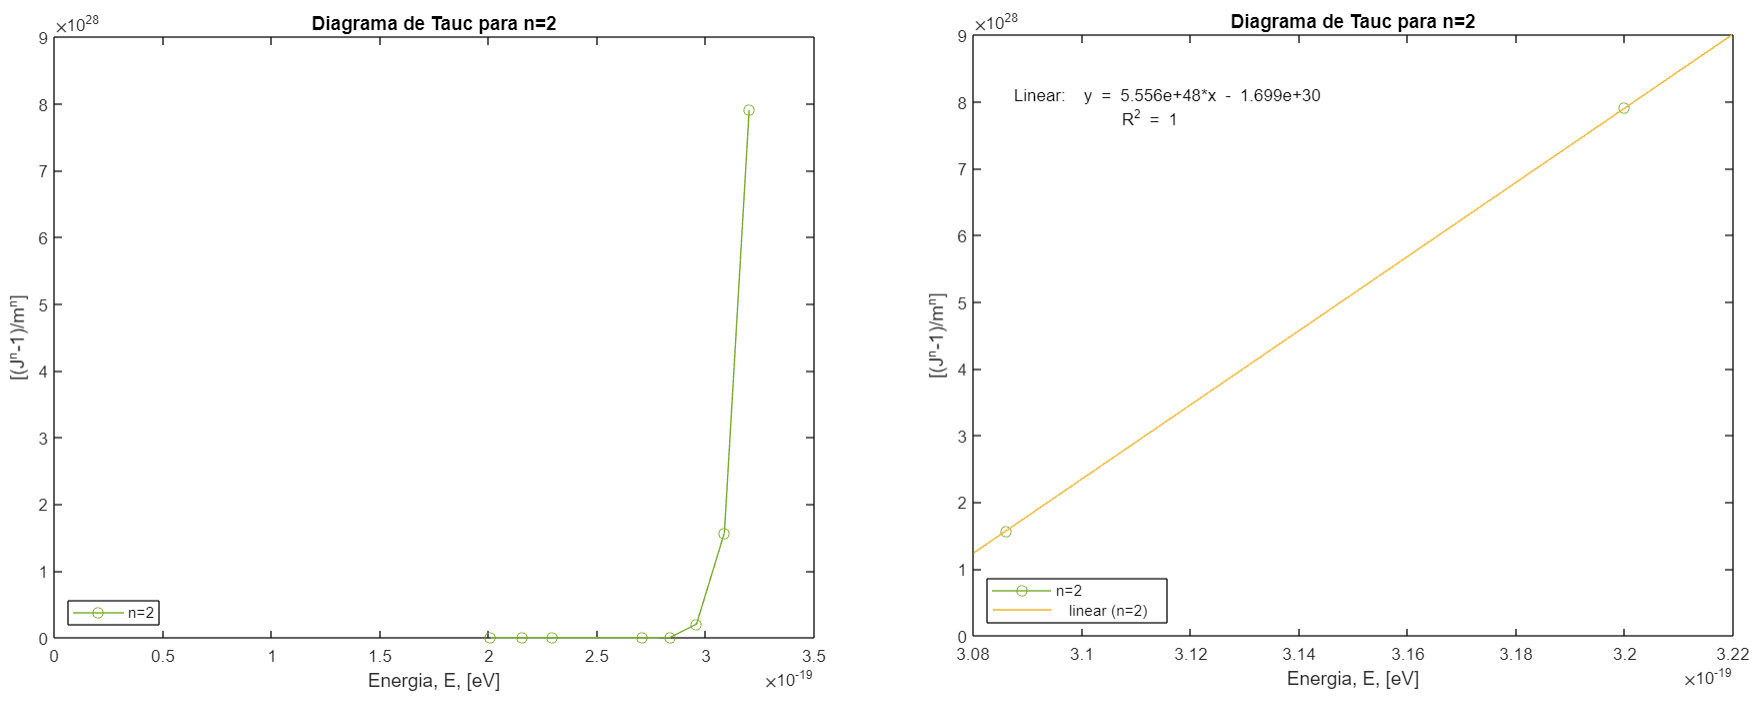
\includegraphics[width=0.75\linewidth]{2-gap.png}
        \caption{ Diagrama de Tauc para exponente $ n=2$. La función de regresión corresponde a $y=53556e+48x-1.699\times10^{30}$ y tiene coeficiente de correlación $R^2=1$.}
        \label{fig:gap 3}
    \end{figure}

        \begin{figure}[H]
        \centering
        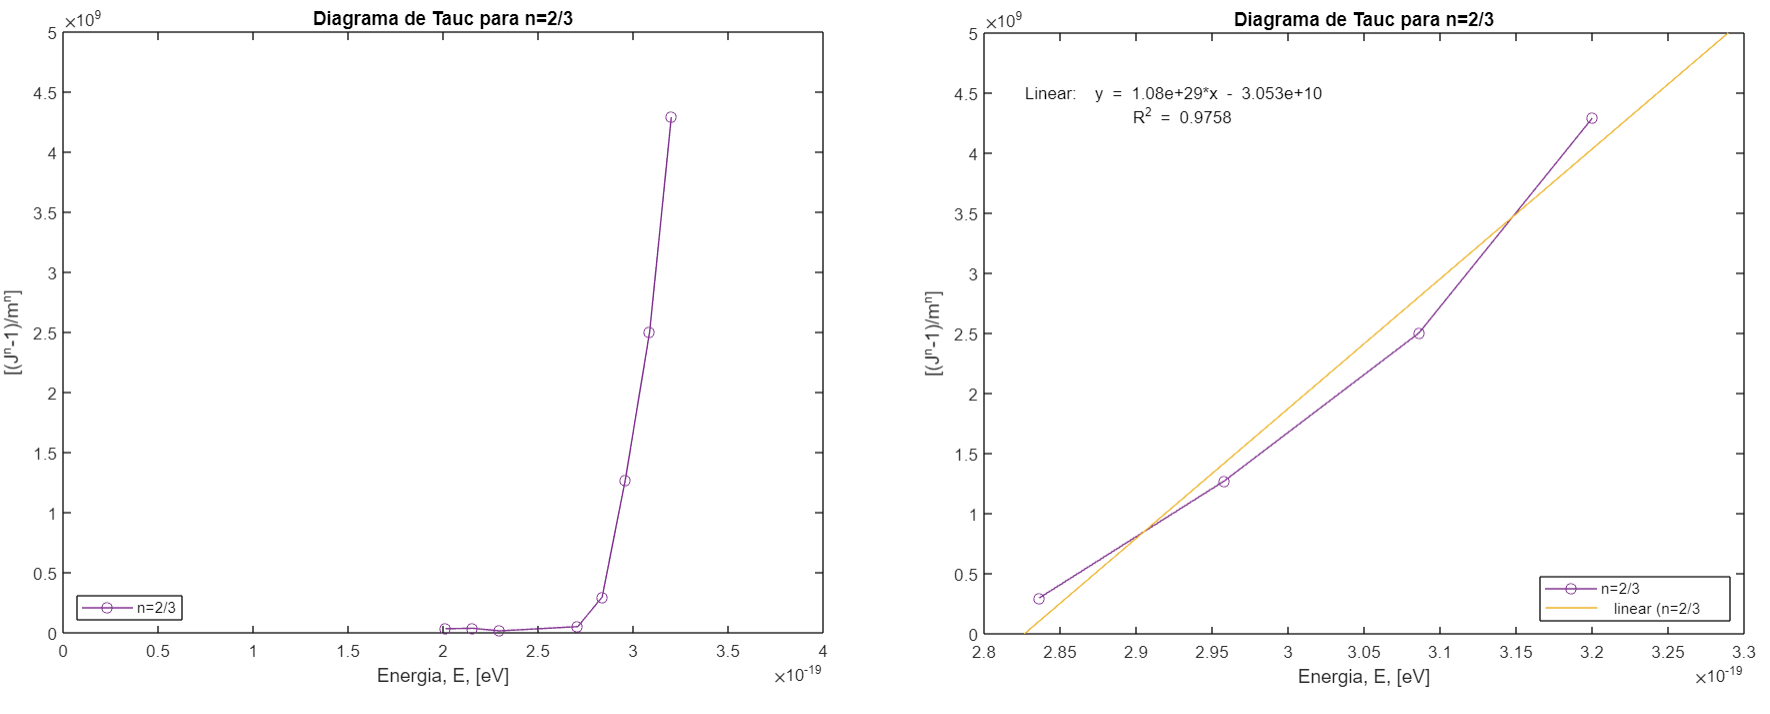
\includegraphics[width=0.75\linewidth]{2_3-gap.png}
        \caption{ Diagrama de Tauc para exponente $ n=\frac{2}{3}$. La función de regresión corresponde a $y=1.08e+39x-3.053\times10^{10}$ y tiene coeficiente de correlación $R^2=0.9758$.}
        \label{fig:gap 4}
    \end{figure}
    
            
    
        
    
\begin{multicols}{2}
     \section{Conclusiones} 
        
        \begin{itemize}
            \item De acuerdo a los resultados obtenidos para el perfil teórico respecto el perfil experimental, se puede concluir que el método de Swanepoel es una excelente manera de obtener los parámetros ópticos de una película delgada únicamente a través de dos cantidades fácilmente medibles en el laboratorio: La longitud de onda incidente y la transmitancia de la película y el sustrato debido a que el proceso de refinamiento a través de los órdenes de interferencia minimiza significativamente la incertidumbre de los parámetros estimados. Esta conclusión se obtiene luego de observar el excelente nivel de concordancia entre los dos modelos dentro del régimen analizado
            
            \item Debido a la razón anterior, también se concluye que el método de Swanepoel funciona muy bien solamente dentro del dominio de los datos analizados, y, por lo tanto, no es extrapolable al dominio de los datos que no pertenecen al conjunto analizado porque esto puede conllevar a estimaciones erróneas. Para refinar el análisis hace falta analizar cuidadosamente los otros regímenes con teorías alternativas o con una metodología más específica diseñada para el análisis de dichos dominios.
            
            \item Con la longitud de onda se obtienen cuatro parámetros fundamentales para describir el sistema sustrato-película delgada; estos parámetros son el grosor $d$ de la película, la función del índice de refracción $n(lambda)$, el coeficiente de extinción $k(\lambda)$ y el índice de refracción del sustrato $s$
            
            \item Comparando los parámetros obtenidos con información de internet, podemos estimar que la película delgada no sólo está hecha de un material amorfo, sino que posiblemente es una aleación que contiene silicio, ya que usualmente las aleaciones de silicio poseen un gap de energía cercano a los $5$ eV y varía según el elemento con el que esté combinado, este valor está dentro del rango de los valores obtenidos.
            
            \item Los distintos exponentes para el banda dieron regiones lineales, por lo tanto se pudo determinar el valor del gap de energía para cada tipo de transición, pero no se puede discriminar entre los datos para determinar qué regiones se dan y qué regiones no, de modo que son necesarios otros experimentos complementarios para determinar estos procesos con más exactitud. Sin embargo el mayor valor de correlación lo presenta el exponente $n=2$, es decir las transiciones directas permitidas asociadas a la brecha de energía de $5.34 eV$.
            
            
            
            
        \end{itemize}
        
        
        
        
        
        
        
        
        
        
        

       
        
       

    


\end{multicols}

\newpage

\section*{Anexos}

\begin{table}[H]
    \centering
    \begin{tabular}{|c|c|c|c|c|c|c|c|}
         \hline $\lambda$ [nm] & $T_m(\lambda)$ & $T_M(\lambda)$ & $n_1(\lambda)$ & $d_1$ [nm] & m & $d_2$ [nm] & $n_2(\lambda)$  \\ \hline
         600&0.4574&0.7962&2.980&1052.8&11&1107.2&2.974\\ \hline
         622&0.4836&0.8603&2.951&1086.2&10+1/2&1106.4&2.943 \\ \hline
         649&0.5019&0.8943&2.916&1140.2&10&1113&2.924 \\ \hline
         677&0.5102&0.9133&2.874&1107.4&9+1/2&1108.6&2.898 \\ \hline
         709&0.5168&0.9133&2.874&1107.4&9&1110.0&2.875 \\ \hline
         746&0.5206&0.9154&2.860&1093.1&8+1/2&1108.7&2.875 \\ \hline
         788&0.525&0.9141&2.839&1105.0&8&1110.4&2.840 \\ \hline
         836&0.52287&0.9147&2.822&1108.9&7+1/2&1110.8&2.825 \\ \hline
         891&0.5324&0.9147&2.807&&7&1111.2&2.810 \\ \hline
         955&0.5355&0.915&2.793&&6+1/2&1111.1&2.797 \\ \hline
    \end{tabular}
    \caption{Valores calculados para los parámetros ópticos $n(\lambda)$ y $d$}
    \label{tab: Datos Refraxión y Película}
    \end{table}
    
    \begin{table}[H]
    \centering
    \begin{tabular}{|c|c|c|c|c|}
        \hline
         $\lambda$ [nm] & $T_M(\lambda)$ & $x(\lambda)$ & $\alpha(\lambda)$ $[nm]^{-1}$ & $k(\lambda)$ \\
         \hline
         600 &0.7962 &09.050 &9.00E-5 &4.30E-03 \\ \hline
         622&0.8603&0.9580&3.87E-05&1.91E-03\\ \hline
         649&0.8943&0.9852&1.34E-05&6.94E-04\\ \hline
         677&0.911&0.9984&1.45E-06&7.81E-05\\ \hline
         709&0.9133&0.9999&9.70E-08&5.47E-06\\ \hline
         746&0.9154&1.0013&-1.19E-06&-7.05E-05\\ \hline
         788&0.9141&1&-2.94E-09&-1.84E-07\\ \hline
         836&0.9144&1&1.32E-08&8.81E-07\\ \hline
         891&0.9147&0.9999&4.76E-08&3.38E-06\\ \hline
         955&0.915&1&3.78E-08&2.87E-06\\ \hline
    \end{tabular}
    \caption{Valores calculados para los parámetros relacionados con la absorción y la extinción}
    \label{tab: Datos x,alpha,k}
    \end{table}
        
    
    
    
\begin{thebibliography}{}

\bibitem{articulo}
R. Swanepoel (1983). \textit{Determination of the thickness and optical constants of amorphous silicon}. Journal of Physics E: Scientific Instruments, 16(12), 1214–1222. \href{http://iopscience.iop.org/0022-3735/16/12/023}{doi:10.1088/0022-3735/16/12/023}

\bibitem{articulo}
F. Mesa , V. Ballesteros
, A. Dussan
\textit{Cálculo de constantes ópticas de películas
delgadas de Cu3BiS3 a través del método de Wolfe}


\bibitem{Local Peaks Tool}
MathLab Documentation. \textit{Find Local Peaks}. MathWorks América Latina. (n.d.). Retrieved June 1, 2022, from \url{https://la.mathworks.com/help/signal/ref/findpeaks.html} 

\end{thebibliography}
\end{document}